%----------------------------------------------------------------------------------------
%	INTRODUCTION
%----------------------------------------------------------------------------------------
\section{Introduction}

Eye tracking is a very common method in cognitive neuroscience and increasingly used in diagnostic medicine, performance monitoring, or consumer experience research.
With increasing demands on the exactness of the eye trackers and growing technical advances, it became possible to record even very small eye movements.
Scientists need to know the performance of an eye tracker, especially because the eye tracker's calibration will deteriorate over time, its accuracy is influenced by luminance changes and biases in the estimated gaze points can be introduced by head movements.


Somebody important said something smart~\citep{thaler_what_2013}.


And now lets have a look at Figures. I am referencing Figure~\ref{fig:RawSignal}.

\begin{figure}[ht]
	\centering
	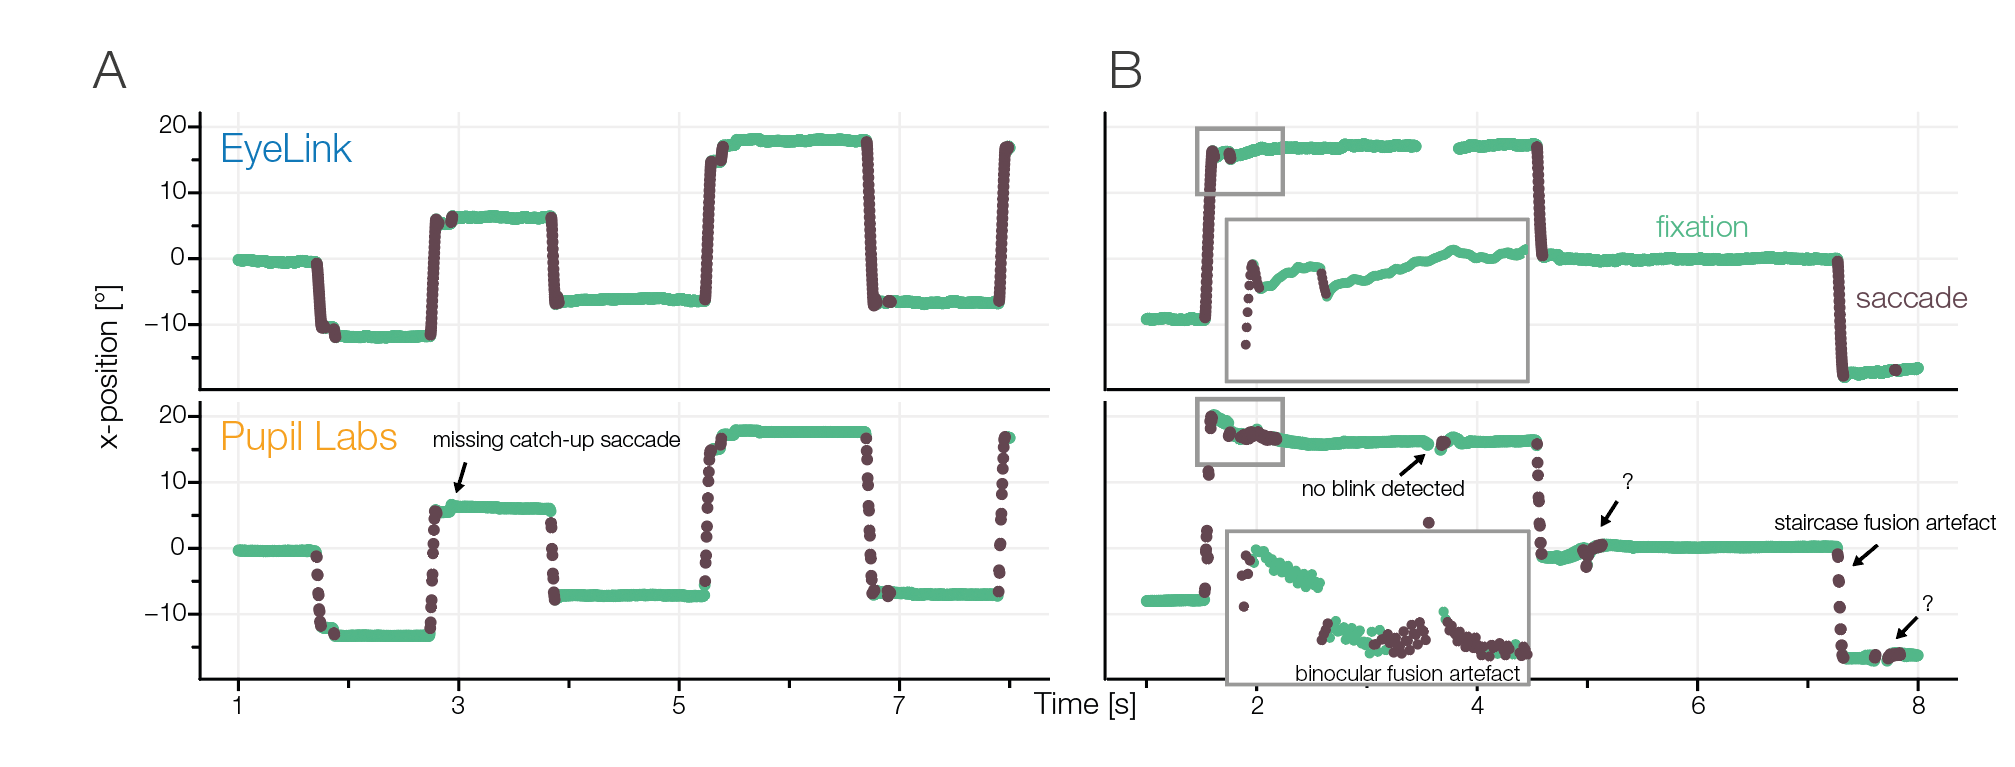
\includegraphics[scale=0.4]{Figures/compare_raw_signal}
	\decoRule
	\caption[Signal of both eye-trackers]{The experiment consisted of six identical blocks. Each block starts with calibration phase and is followed by a fixed sequence of the ten conditions. Thus, each participant took part in six calibration procedures and a total of 60 conditions.}
	\label{fig:RawSignal}
\end{figure}

Add the image to the Figures folder.
